\documentclass{article}
\usepackage[utf8]{inputenc}
\usepackage[margin=1in]{geometry}
\usepackage{graphicx}
\usepackage{subcaption}
\usepackage{amsmath}
\usepackage{hyperref}
\setlength{\parindent}{0em}
\setlength{\parskip}{0.5em}
\title{Assignment 3}
\author{Amalia Karalis}
\date{May 2022}

\title{Assignment 3}
\author{Amalia Karalis}
\date{}

\begin{document}

\maketitle
\section*{Question 1}
In question 1, the python file complex\_iter.py contains a function that takes in the initial value for z, the grid size of the complex plane (i.e. the number of points to consider in the complex plane $c = x+ iy$, for $-2 < x < 2$ and $-2 < y < 2$) and the number of iteration of z.
The functions iterates the equation the equation $z_{i + 1} = z_i^2 + c$ at each point in the complex plane and returns the X grid, the Y grid, the values of z at each iteration for each point in the grid, and the value at which, if any, z diverges.

This function is used to produce a plot of the complex plane showing the points that diverge in red triangles and the points that remain finite in black circles. An example of such a plot is shown in the left plot of Figure \ref{fig: Divergence_z_cplane}. We also note the iteration at which the value of z diverges, which is returned by the function complex\_iter in the array div\_iter. If z does not diverge within the given number of iterations, the array returns a NaN at that point in the plane. This is used to plot a colormap indicating the value at which the points on the complex plane diverge, an example of which is shown in the right panel of Figure \ref{fig: Divergence_z_cplane}. 

\begin{figure}[ht!]
    \begin{minipage}{0.48\linewidth}
    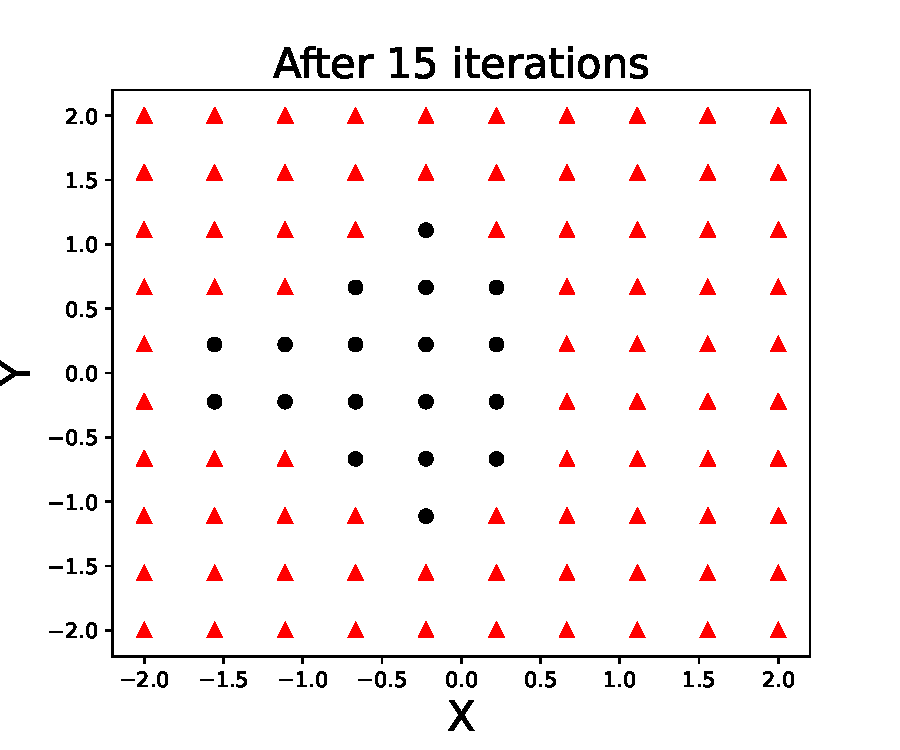
\includegraphics[scale = 0.5]{Q1_Fig1.pdf} 
        \centering
    \end{minipage}
    \begin{minipage}{0.48\linewidth}
        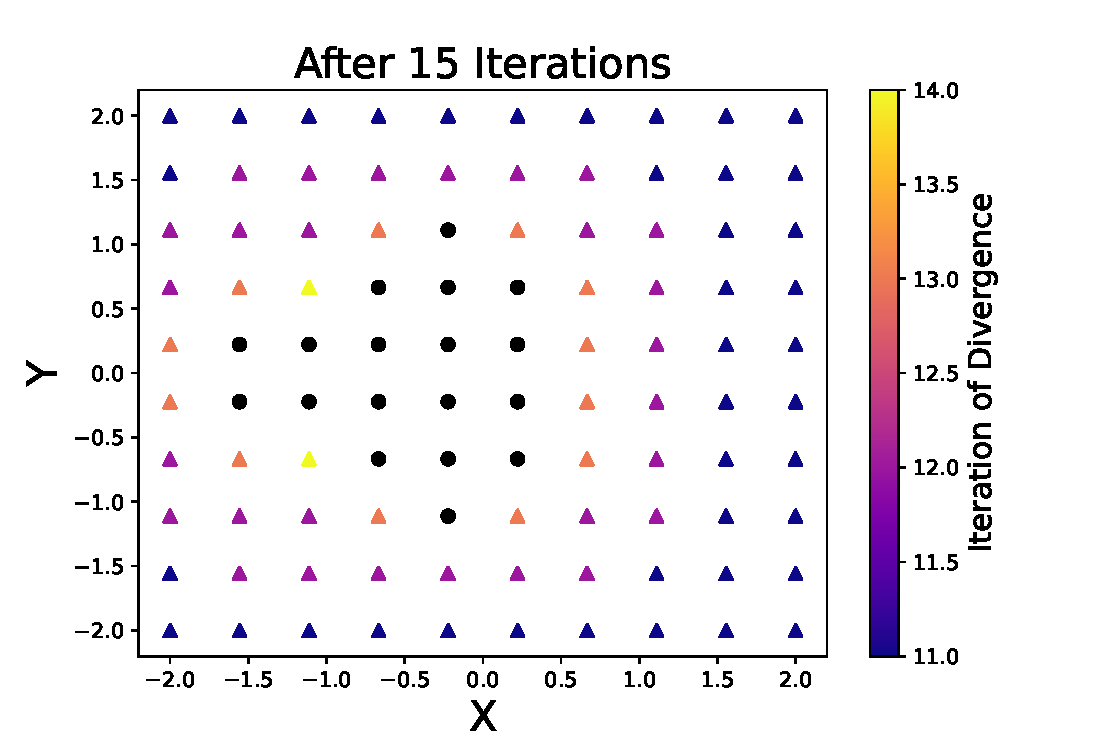
\includegraphics[scale = 0.5]{Q1_Fig2.pdf}
        \centering
    \end{minipage}
    \caption{The divergence of z in the complex plane. Right: After 15 iterations of z, the points in the complex plane for which z diverges are plotted as red triangles, and those that remain finite are plotted as black circles. Right: Same as left, but with a colorbar showing the iteration at which the divergence of z happens.}
    \label{fig: Divergence_z_cplane}
\end{figure}


\section*{Question 2}
In question 2, we define a function W\_dot, the three coupled ordinary differential equation that describe convection (the convection equations). This function takes t, the dimensionless time parameter, W = [X, Y, Z], and params = [$\sigma$, r, b], where $\sigma$ is the Prandtl number, r is the Rayleigh number and b is an dimensionless length scale and returns [$\dot{X}$, $\dot{Y}$, $\dot{Z}$], the ODEs as defined in Equations 25, 26 and 27 of Lorentz (1963). The ODEs solver \texttt{solve\_ivp} from \texttt{scipy.integrate} is used to solve these coupled differential equations, with initial values  $W_0=[0., 1., 0.]$ and parameter values [$\sigma, r, b$] = [10., 28, 8./3.], taken from Lorentz (1963).
Using this, we can reproduce Figure 1 from Lorentz (1963), which is shown in Figure \ref{fig:Lorentz_fig1}. Figure 2 from Lorentz (1963) was reproduced by solving the differential equations over a time range from 14 to 19, and plotting the results. Figure \ref{fig:Lorentz_fig2} shows the numerical solutions to the convection equations projected in the Y-Z plane (top) and in the X-Y plane (bottom).

\begin{figure}[h]
    \centering
    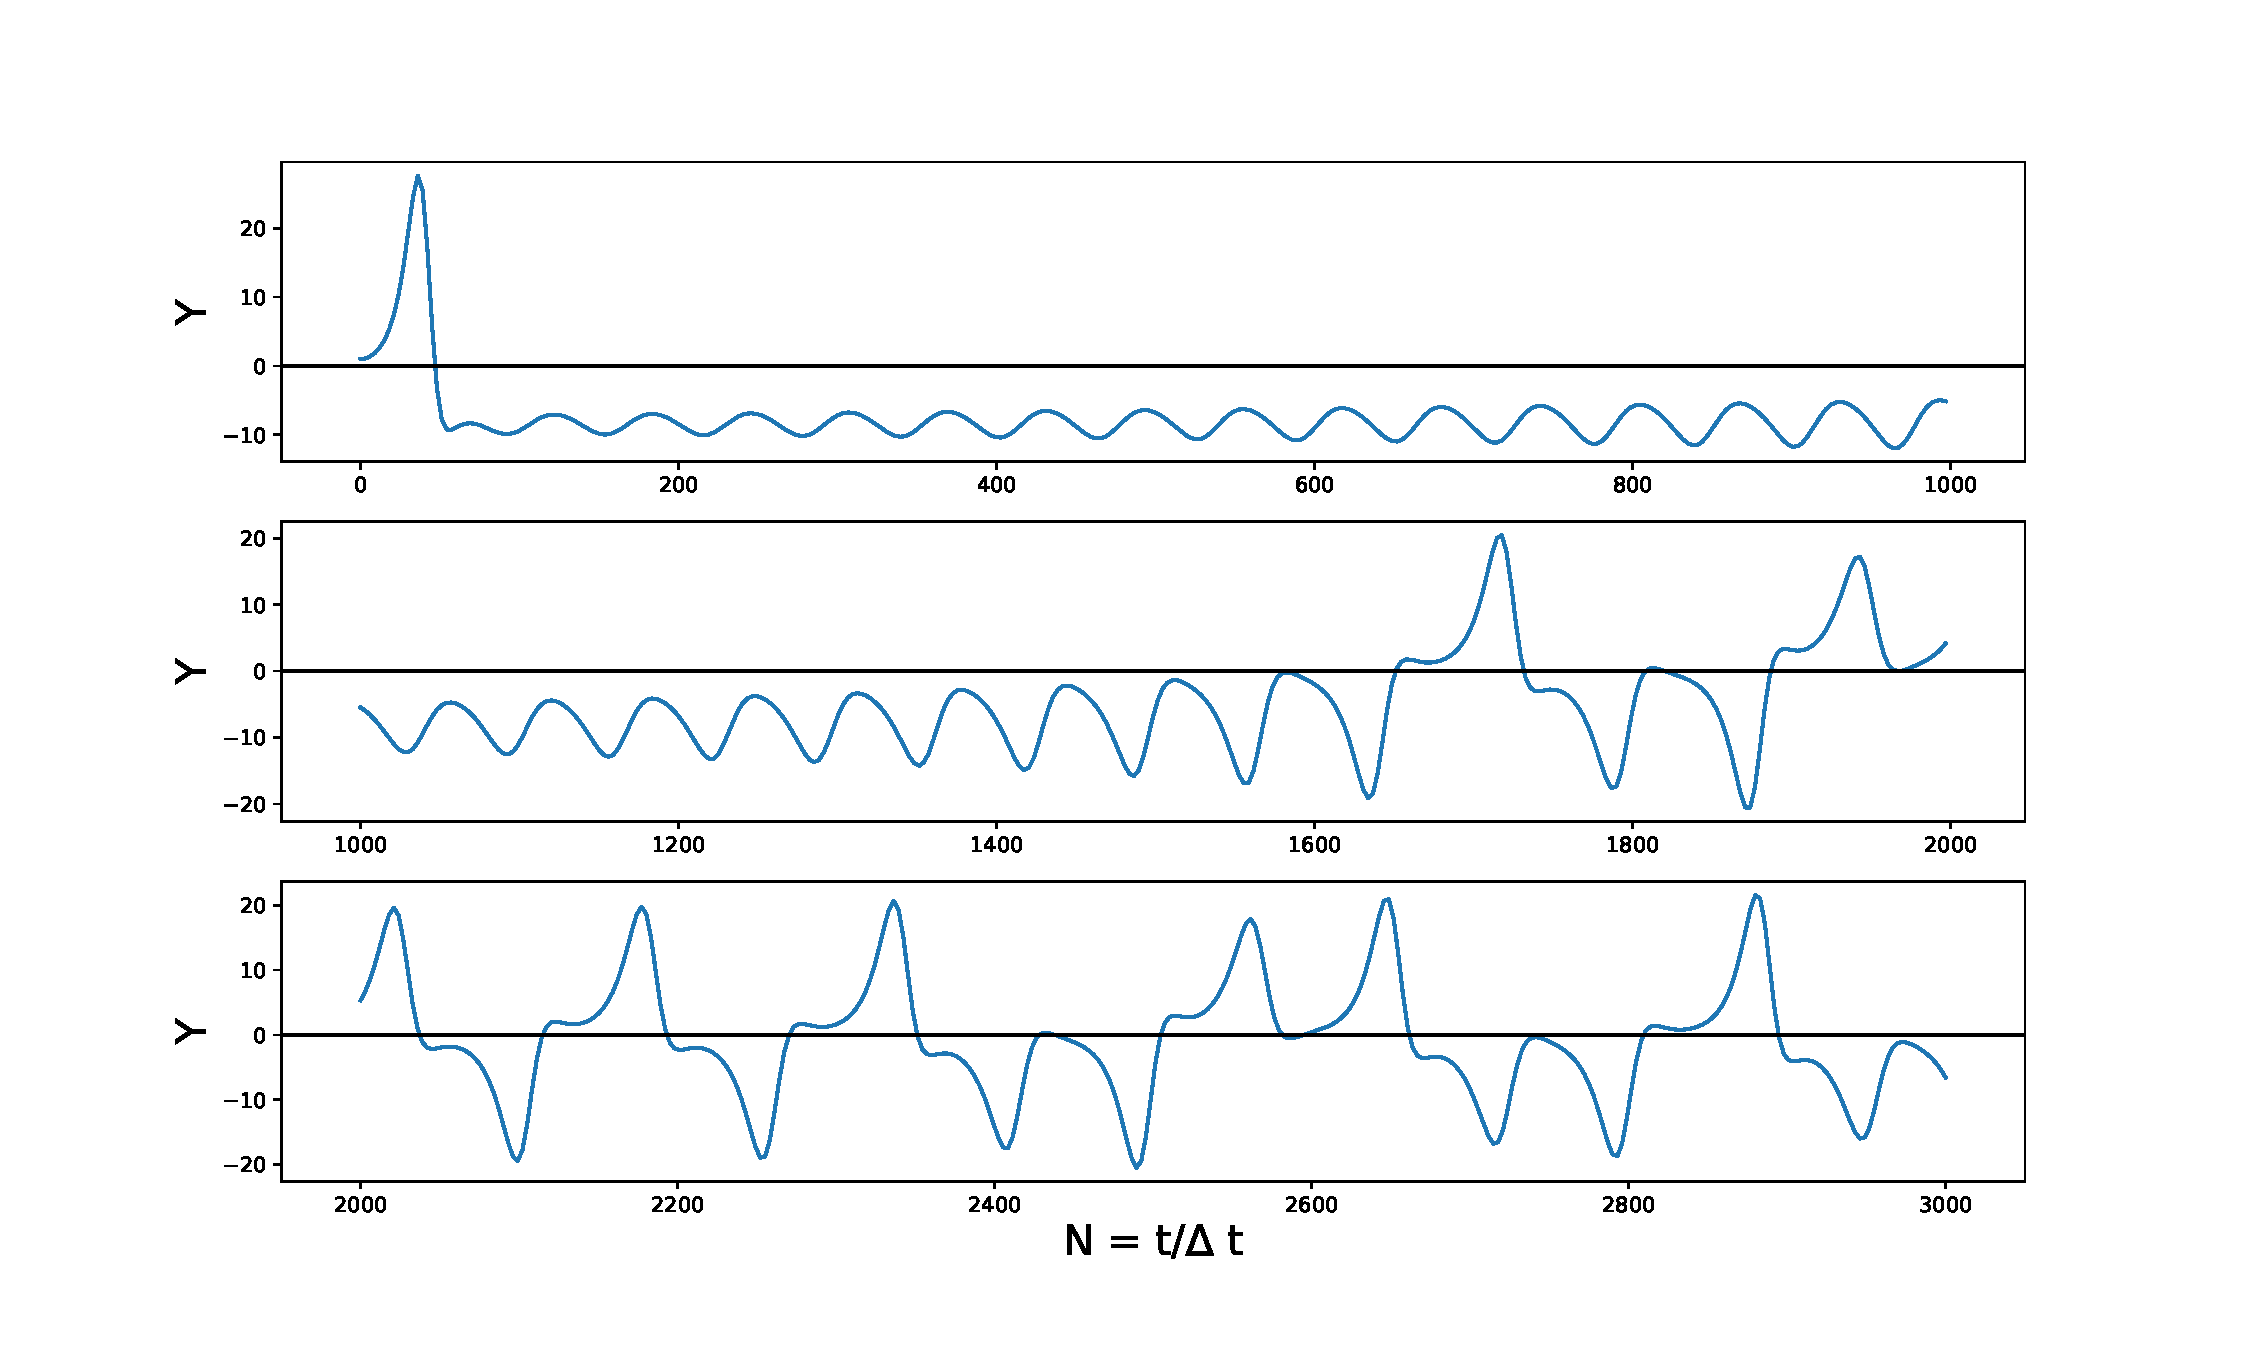
\includegraphics[scale=0.4]{Lorentz_fig1.pdf}
    \caption{Y as a function of N, the iteration number of the ode solver, where N=t/$\Delta$t, t the dimensionless time parameter and $\Delta t =0.01$ for the first 1000 iterations (top), the second 1000 iterations (middle) and the third 1000 iterations (bottom).}
    \label{fig:Lorentz_fig1}
\end{figure}

\begin{figure}[ht!]
    \centering
    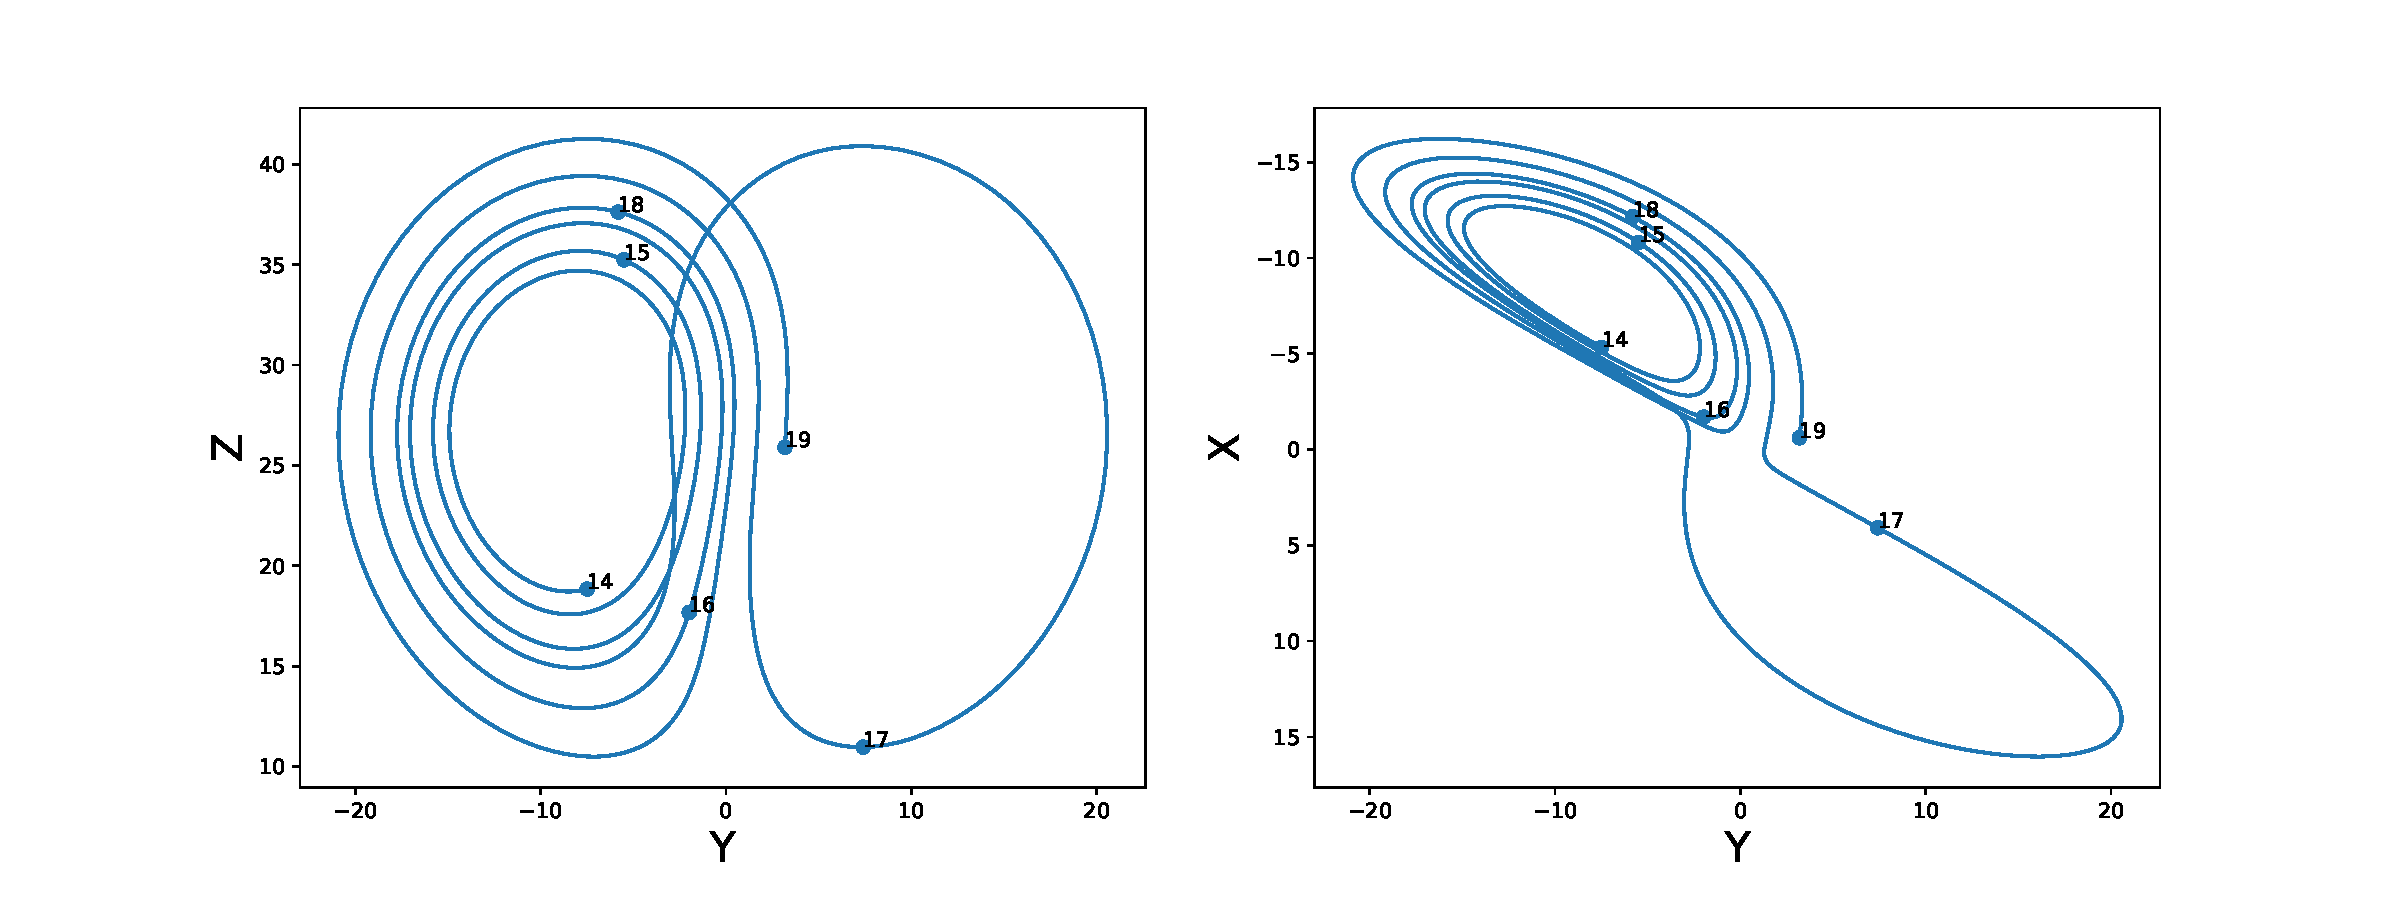
\includegraphics[scale=0.4]{Lorentz_fig2.pdf}
    \caption{Numerical solutions to the convection equations projected in the Y-Z plane (top) and in the X-Y plane (bottom).}
    \label{fig:Lorentz_fig2}
\end{figure}



\begin{figure}[ht]
    \centering
    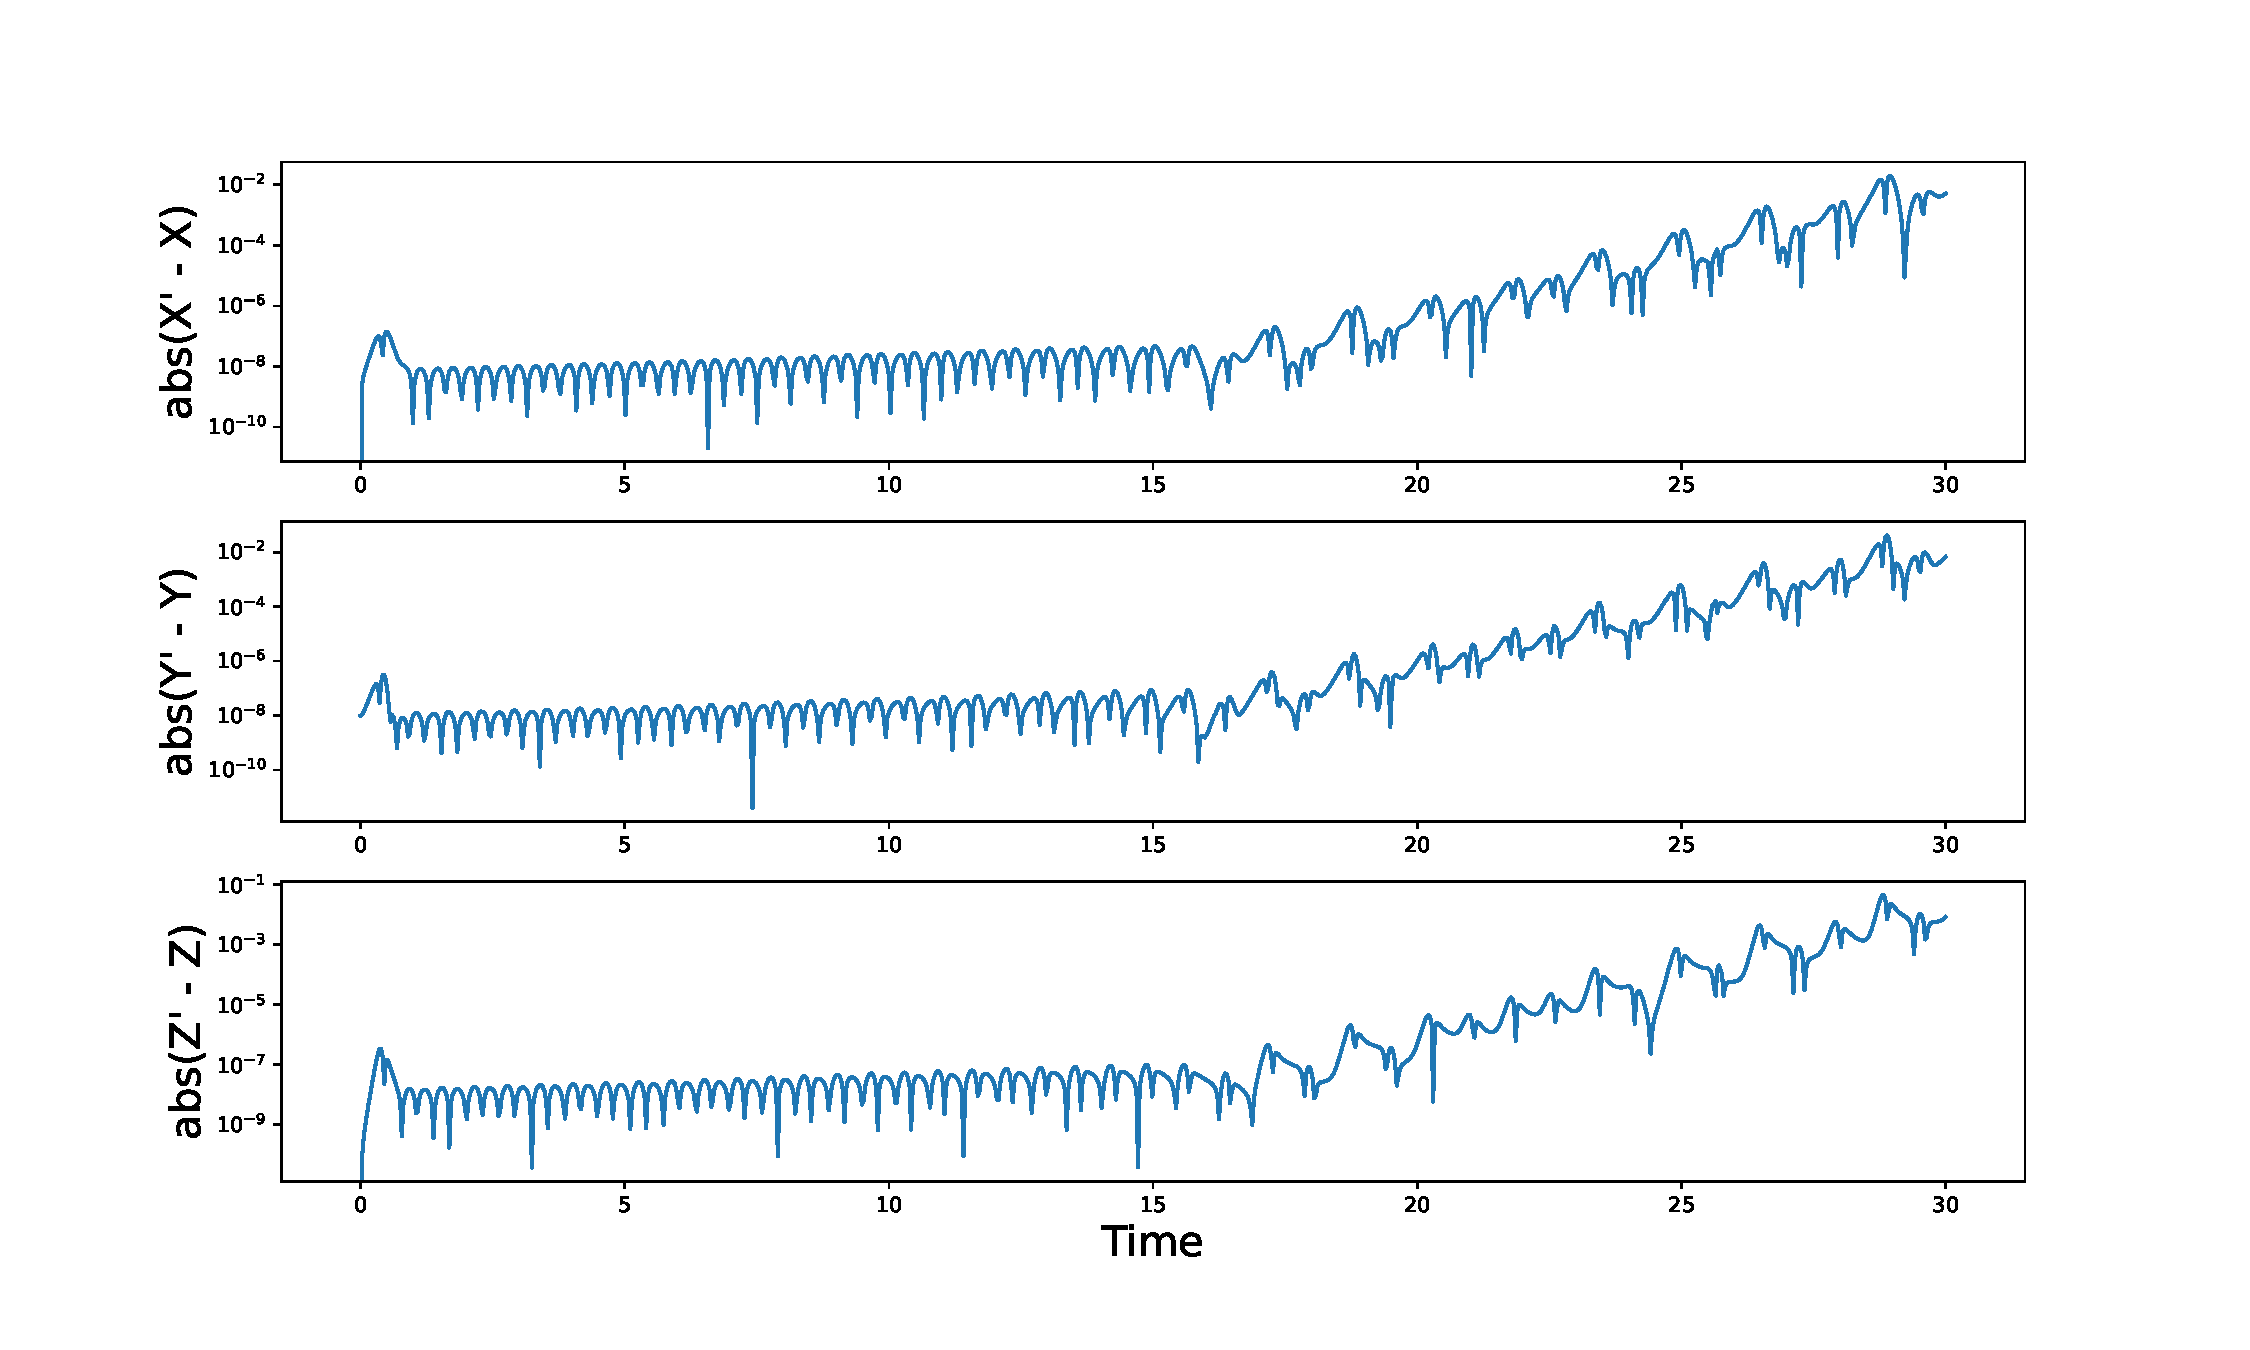
\includegraphics[scale=0.4]{Error_plot.pdf}
    \caption{The absolute difference in the two solutions as a function of time, where the initial condition in Y is varied slightly from 1.0 in W to 1.00000001 in W'.}
    \label{fig:error_plot}
\end{figure}

This method was redone using slightly different initial conditions: $W'_0 = W_0+[0., 1.e-8, 0] = [0., 1.00000001, 0.]$. We show the difference in the solutions obtained in Figure \ref{fig:error_plot}

\end{document}




